%!TEX root = ../main.tex

\chapter{Design of a New Model}
\label{chp:design}

In this chapter, we will introduce our static word embedding model by describing its background and architecture, and highlight its differences with respect to the state-of-the-art models in the literature.

\section{Preliminaries}
We will begin by establishing the fundamental symbols and concepts that will be employed throughout this chapter. 

\begin{itemize}
\item We consider the vector space $V = R^N$.
\item $T$ is a generic text used in the training process.
\item $u, v, w, u_1, . . .$ denote words appearing in $T$. Each individual word may have multiple occurrences in $T$, at different positions.
\item We use $p$, ${p}'$ to denote positions.
\item For a word $w$, $C(w)$ is the set of words appearing in $T$ in the context of $w$, that is, words that are found at some bounded distance from any occurrence of $w$ in $T$.
\item For each word $w$, $e_t(w)  \in V$ denotes a target vector embedding for $w$, and $e_c(w) \in V$ denotes a context vector embedding for $w$. 
\item $\tau$ is the target embedding matrix, and $\varsigma$ is the context embedding matrix.
\end{itemize}

Also, it will be useful to introduce beforehand some mathematical operations we will encounter later on.

\subsection{Sigmoid}
\label{sec:sigmoid}

The sigmoid function (or the logistic function) is a mathematical function that is used to map any real number to a value from the range defined between 0 and 1. When plotted, it has an S-shaped curve, which is the reason for its name. It is a popular and multipurpose function in the machine learning domain as it introduces non-linearity into models.

Sigmoid is a popular choice for making predictions in binary classification problems. It is a useful way of calculating the probability that an input belongs to one of the two classes. Sigmoid provides smooth transitions between the two extremes (0 and 1). In neural networks, the sigmoid function was historically used as an activation function in the hidden layers.

The sigmoid function is defined as:
\[ \sigma(x) = \frac{1}{1 + e^{-x}} \]

Where $x$ is the input, which can be any real number. Figure \ref{fig:sigmoid} visualizes the sigmoid function.

\begin{figure}[H]
    \centering
    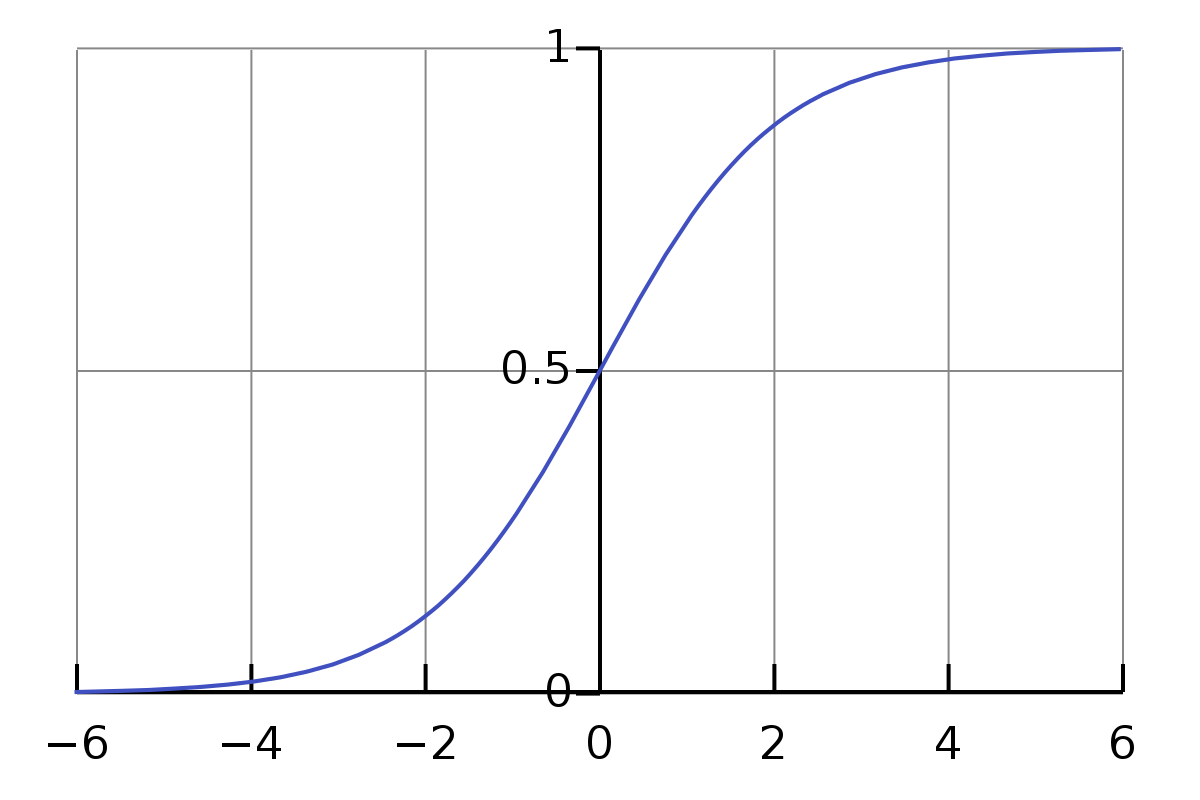
\includegraphics[width=0.6\textwidth]{img/sigmoid.png}
    \caption{Sigmoid function}
    \label{fig:sigmoid}
\end{figure}

We will use $\sigma$ for denoting the sigmoid function throughout this chapter.

\subsection{ReLU}

\ac{ReLU} is a widely used activation function in machine learning systems, especially in neural networks. \ac{ReLU} is a simple yet effective activation function that clamps negative values to zero and yields the input value as it is for non-negative inputs. It is computationally efficient, given that it is essentially a simple thresholding operation, making it faster to compute and more feasible for lower-end computing units. Thanks to its simplicity and non-linearity, it became the standard choice for many artificial neural networks.

The \ac{ReLU} function is defined as:
\[
\text{ReLU}(x) = \max(0, x)
\]
\noindent
where $x$ is the input, which can be any real number.


\subsection{Softplus}

Now we will present the softplus function, which is another mathematical function often used in machine learning. It is a smooth and differentiable unbounded function that maps any real number to a positive value.

The softplus function provides a smooth alternative to \ac{ReLU} and its variants (like Leaky-\ac{ReLU}). While \ac{ReLU} is a popular choice, especially as an activation function in deep neural networks, its behavior of mapping any non-positive value to zero might introduce problems in some settings. Readers are encouraged to have a look at \cite{softplus} for a better intuition for why the softplus function can be a better choice in some deep learning tasks, and why \ac{ReLU} is still a more popular option.

The softplus function ($\varsigma$) is defined as:

\[ \varsigma(x) = \ln(1 + e^x) \]
\noindent
where $x$ is the input, which can be any real number. In Figure \ref{fig:softplus}, we visualize the softplus function and compare it to the \ac{ReLU}.

\begin{figure}[H]
    \centering
    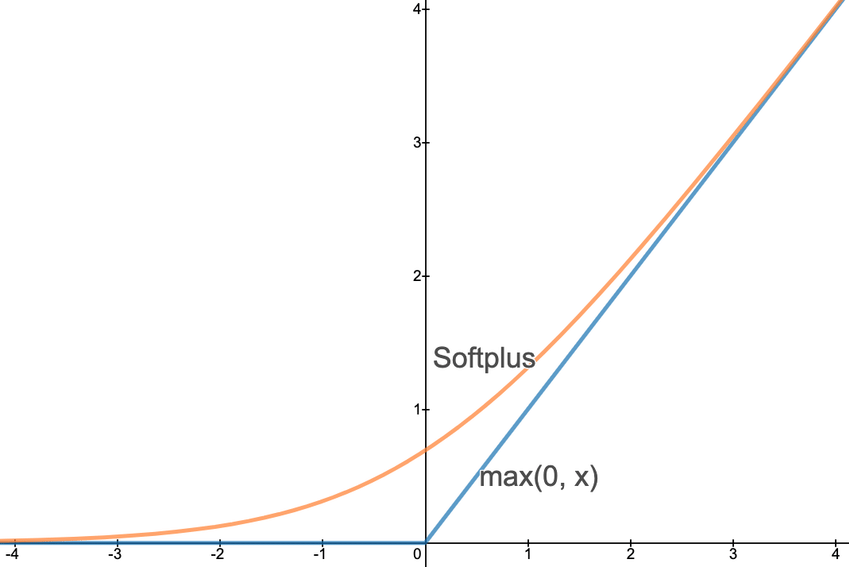
\includegraphics[width=0.6\textwidth]{img/softplus.PNG}
    \caption{Softplus function, compared to \ac{ReLU}}
    \label{fig:softplus}
\end{figure}

We will use $\varsigma$ for denoting the softplus function throughout this chapter.


\section{SGNS: Geometrical point of view}
Before sharing our idea of organizing embedding vectors in a vector space, it will be useful to first briefly introduce our understanding of the configuration learned by the \ac{SGNS} model. 

Let $w$ be a target word. The target of the \ac{SGNS} imposes that for every word $u \in C(w)$, $e_c(u)$ forms a “small” angle with $e_t(w)$.
This suggests the existence of an \textbf{N-dimensional cone} surrounding $e_t(w)$, and every $e_c(u)$ is contained in such cone. Coming from this, the model enforces words with similar contexts to have overlapping cones, hence the small angle between their target representations. This way, the model performs well in cosine similarity-based similarity tasks.

For describing this geometrical configuration based on the idea of context cones, a toy example in three dimensions may be useful. For this purpose, we prepared a figure visualizing how we expect the learning process to arrange context and target representations based on word occurrences. We imagine three target words: $w_1$, $w_2$ and $w_3$. For this example, imagine that $w_1$ and $w_2$ are two words that share similar contexts in $T$, whereas $w_3$ is not so related to the other two. Based on the training objective of \ac{SGNS}, we understand that we can expect to see a configuration similar to the one given in Figure \ref{fig:cones}.


\begin{figure}[ht]
    \centering
    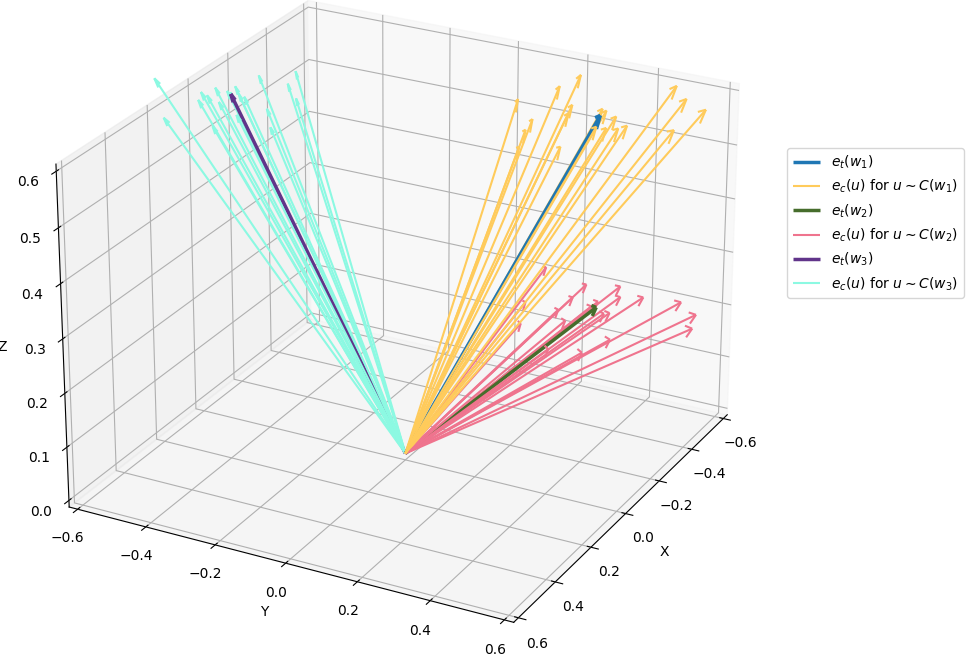
\includegraphics[width=0.9\textwidth]{img/context_cones.png}
    \caption{Context cones for three target words in three dimensions.}
    \label{fig:cones}
\end{figure}


In this figure, we highlighted the cone-like distribution of context word samples around the target word and the shared contexts of $w_1$ and $w_2$, hence the overlapping context cones. Thanks to this, it is easy to see that these two words will have greater cosine similarity than any other combination, and based on the distributional hypothesis, this is exactly what is desired. One should note that, however, this is just a visual prepared manually to assist the reader in following our intuition, and it will not be nearly as straightforward to observe similar shapes and distributions in a real training setting, given factors such as the high dimensionality, the size of the vocabulary and the noise.

Different models using different targets will yield either different geometrical configurations, or obtain similar results with different techniques. This is essentially what makes a model novel and the difference in the final configuration is what makes a model "better" in a task than some other model.

\section{Our model}
In this study, we propose a novel neural static word embedding model that is learned using orthogonal projections of vectors to represent contextual relationships. Many models, such as \ac{SGNS}, aim to capture contextual relationships of words based on one-to-one co-occurrences. Meanwhile, our model employs a third-order approach and leverages the contrastive learning paradigm, in which a positive training sample consists of a target word and two context words, and a negative sample consists of one target word, one context word, and a randomly sampled noise word from the corpus. This approach is distinct from the traditional static embedding models, and results in word embeddings that effectively capture contextual information in a higher-order, projective manner. 

We developed a unique geometrical loss function that aims to minimize the difference between the orthogonal projections of the selected context words onto the target word and maximize the difference between the orthogonal projections of the context word and the negative samples onto the target word.

We designed the training procedure using a neural network. Just like in \cite{w2v2}, we used two embedding matrices and we tuned these matrices as the weights of this feedforward network by backpropagating the gradients of our loss function.

\section{Design choices}

In developing our model and designing the training pipeline, we needed to make certain choices, and each decision needed to be carefully analyzed in order to maximize the performance of the final model. Some of these decisions needed to rely on other works, but some of them needed to be tested out for our specific needs.

\subsubsection{Number of embedding matrices}

We first investigated whether or not it is logical to use two embedding matrices, just like how they proposed in word2vec \cite{w2v2}. They use two representations for each word $w$, $e_t(w)$ and $e_c(w)$. $e_t(w)$ is the target embedding of $w$ which is the final product, and $e_c(w)$ is the context embedding, which is only used during the training. We have trained an \ac{SGNS} model with an implementation found online, using both single-embedding and two-embedding approaches. The results indicated the benefit of two embeddings. We were convinced that the same would apply to our model as well since both models leverage the contrastive learning paradigm.

%\subsubsection{Embedding dimensions} % Move this section

%The embedding dimension is yet another thing that directly influences the final performance. It is the factor that sets the amount of information that can be stored in an embedding vector. Based on this, we found that the dimension of 300 is quite a common choice in the literature, and it is a good number for our memory and processing resources.

\subsubsection{Negative samples} 

Our model's loss function works on both negative and positive samples, this means for a target word $w$, we need its context words $C(w)$ for positive training samples. On the other hand, $C(w)$ and $w_n$ are needed for a negative training sample, where $w_n$ is a noise word randomly sampled from the training corpus. \cite{w2v2} uses a factor $k$ which is the number of negative training samples for each positive training sample. It is the common practice to keep this number greater than one. 

As for the sampling of the $w_n$ for each negative training sample, the natural idea would be picking a random word from the vocabulary, following a uniform probability distribution. But we again decided to follow the findings reported in \cite{w2v2} and work with a sampling table. In this technique, based on the word occurrence frequencies, we generate a sampling table and we pick a $w_n$ from this table at random. A word appears on this table many times which is proportional to its frequency, which can be expressed as follows: 

\[m_w = \frac{f_w^{0.75}}{Z}\]
\noindent
where $m_w$ is the number of times a word occurs on this sampling table, $f_w$ is the number of occurrences of this word in the vocabulary, and $Z$ is computed as follows:

\[Z = \sum_{w}^{V} f_w^{0.75}\]

\subsubsection{Positive samples}

For generating training samples, we needed to obtain the contexts of each target word. The context of a word occurrence is the set of words that appear at a limited distance from that target word occurrence. For this purpose, one needs to set a parameter $L$, which is the size of the context window. The context is collected for a target occurrence from the $L$ distance on the left and right of the target word. For instance, for a fixed window implementation, let us fix the parameter $L$ to 2 and target $w$ as "\textit{web}". In the following sentence:

\begin{displayquote}
Many desktop publishing packages and \underline{web} page editors now use Lorem Ipsum as their default model text.
\end{displayquote}

If we use a string preprocessing to eliminate conjunction, $C(w)$ consists of: "\textit{publishing, packages, page, editors}". These are the words that we can easily associate with the meaning we derive from the word "\textit{web}". If we change our mind and set $L=4$, now $C(w)$ consists of: "\textit{many, desktop, publishing, packages, page, editors, now, use}". Even though we can still associate these words with "\textit{web}", it is easy to see that as we extend the window size, we will come across words that are less strictly related to our target word. This might introduce noise to our learning but also enable us to learn more far-sighted relations of words. Coming from this, we needed to be mindful while choosing the window size, as it would directly influence the relations of the word representations.

What we described above links with an approach called "\textit{Fixed-Sized Context Window}". We combine this with another approach, "\textit{Dynamic Context Windows}", to add a bit of randomness to it.

Dynamic context windows approach is a way of leveraging the advantages of multiple window sizes throughout the training. Based on some factor, or completely at random, one can keep changing the size of a context for each training sample. We decided to follow this approach and picked the window size from $[2, L+1]$ for each sample at random. By keeping this dynamic range dependent on the pre-defined parameter $L$, we keep control of more or less how many words are to be collected on average from each context window, but still leveraging from the randomness that comes from the dynamic approach.

\section{3rd order loss}
\label{sec:loss}

For any machine learning model, the loss function is the main factor that determines the characteristics and the purpose of the model by setting the objective. Word embedding models are no exception, depending on the loss function used, the embedding models can be enabled to capture complicated contextual relationships of words with increasing accuracy, in order to succeed in downstream tasks.

When we decided to work with a third-order structure, our objective was capturing contextual relationships in a higher order, with the aim of obtaining vectors encoding more complex relationships than what can be captured with traditional models. 

Throughout our study, we continuously made changes to our loss function and reported the results. In this section, we will talk about our "base" model, which was our starting point when we implemented a new loss function. More about the specifications of our base model and how its variants differ from it will be explained in Chapter \ref{chp:experiments}.

\begin{figure}[ht]
    \centering
    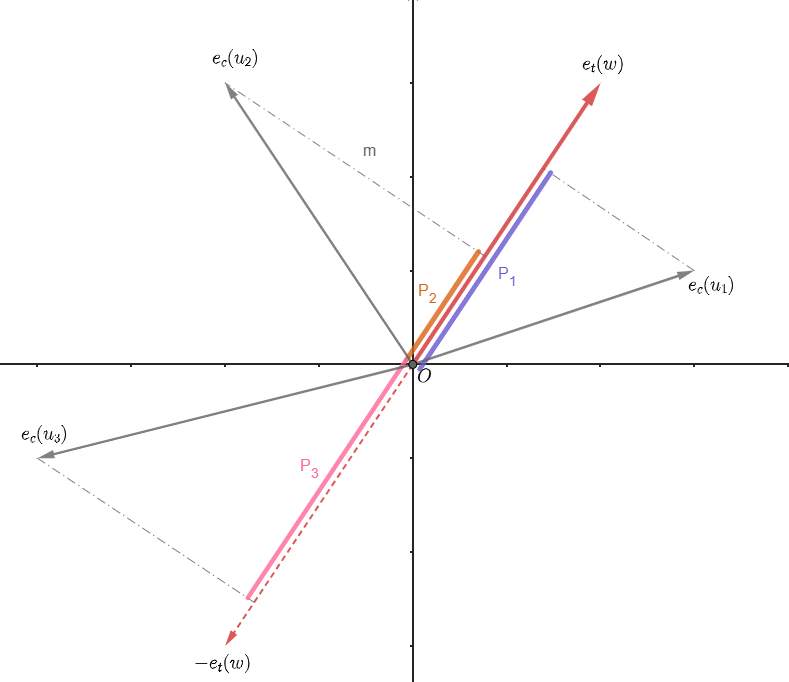
\includegraphics[width=0.8\textwidth]{img/loss_plot.png}
    \caption{One target and three context embedding vectors, and orthogonal projections onto the target vector.}
    \label{fig:loss_plot}
\end{figure}

Let us describe the objective of our training using Figure \ref{fig:loss_plot}. Here, we see four vectors for four words, $w, u_1, u_2, u_3$. $w$ is our target word, we show its target embedding vector. The rest are other words sampled from the vocabulary, and we see their context representations. As we said earlier, our loss function is based on orthogonal projections, therefore we also show the orthogonal projections of these context representations onto the target representation of $w$, $e_t(w)$.

Dotted lines connecting context vectors to the target vector visualize the projections. Colored lines show the magnitude of the orthogonal projections. $P_1, P_2, P_3$ visualize the magnitudes of the orthogonal projections of $u_1, u_2 , u_3$ respectively, onto the target representation of $w$.

Our loss function has two components. Let us imagine training samples, using the vectors in Figure \ref{fig:loss_plot}. One positive sample, $(w, u_1, u_2)$, consists of a target word and two context words sampled from the context window of one occurrence of the target word. And one negative sample, $(w, u_1, u_3)$, consisting of one target word, one context word, and a noise word sampled from the vocabulary. Using these, the components of the loss function are:

\begin{itemize}
\item \textbf{Positive Loss $\myscore{+}{w, u_1, u_2}$:} Forces context words $u_1$ and $u_2$ to have similar projections onto the target $w$. Uses positive training samples. Penalizes the projection difference of the context embeddings of two context words, $e_c(u_1)$ and $e_c(u_2)$ onto the target representation of the target word, $e_t(w)$. In other words, aims to minimize $| P_1 - P_2 |$.
\item \textbf{Negative Loss $\myscore{-}{w, u_1, u_3}$:} Uses negative training samples. Aims to push the noise projection to the left side of the context projection, onto the target vector. In order words, aims to maximize $P_1 - P_3$.
\end{itemize} 

Overall loss $L$ is calculated for our two training samples as:

\[L = - \left ( \log{\myscore{+}{w, u_1, u_2}} + \log{\myscore{-}{w, u_1, u_3}} \right )\]
\noindent
We use $\log$ for a more efficient convergence since both positive and negative loss yield small values. Generalizing this formula for every training sample generated for each word in the vocabulary:

\[L = - \sum_{w \in V} \left (\sum_{u_1, u_2 \in C(w)} \log{\myscore{+}{w, u_1, u_2}} + \sum_{u_1 \in C(w), u_3 \sim S, u_3 \notin C(w)} \log{\myscore{-}{w, u_1, u_3}}\right )\]

Where $S$ is our negative sampling table.

\subsection{Positive loss}

Now we will have a closer look at the computation of the positive loss, $\myscore{+}{w, u_1, u_2}$. We will continue using our example positive training sample $(w, u_1, u_2)$ from Figure \ref{fig:loss_plot} in our descriptions.

As we discussed earlier, this part of our loss aims to minimize the projection difference of context representations of the context words onto the target representation of the target word. In other words, our goal is to minimize $| D = P_1 - P_2 |$. $D$ is calculated as follows:

\[ D = \frac{e_c(u_1) \cdot e_t(w) - e_c(u_2) \cdot e_t(w)}{\left \| e_t(w) \right \|}\]

Using $D$, the calculation of $\myscore{+}{w, u_1, u_2}$ is:

\[ 
\myscore{+}{w, u_1, u_2} = 2 \cdot (\sigma( \varsigma  (D) ))
\]
\noindent
where $\sigma$ is the sigmoid function and $\varsigma$ is the softplus function.

By applying the softplus function to $D$, we first ensure that $P_1 - P_2$ is positive. It will fix the negative values to a positive value near zero. We went with softplus instead of \ac{ReLU}, because softplus is continuous and differentiable everywhere unlike \ac{ReLU}, and almost as resource-efficient. Nevertheless, we still tested this decision by employing \ac{ReLU} in another version of our model (see Section \ref{sec:variants}), and the results proved the superiority of softplus. Not learning from the samples where $D$ is a negative value might seem like a loss of information, however, we should note that the existence of a positive sample $(w, u_1, u_2)$ ensures the existence of another positive sample $(w, u_2, u_1)$ thanks to our implementation of the sampling procedure.

Next, this value is passed through a sigmoid operation, and this yields a probability. Then, it is multiplied by two, so that the impact of the positive loss is amplified. We decided this was needed because the negative loss was dominating the positive loss, considering that the negative loss is calculated for five samples per one positive sample.

\subsection{Negative loss}
\label{sec:neg_loss}

Next, we describe the computation of the negative loss, $\myscore{-}{w, u_1, u_3}$. We are still proceeding with our example negative training sample $(w, u_1, u_3)$ from Figure \ref{fig:loss_plot}.

This part of our loss aims to maximize the projection difference of context representations of the context words and the context representation of the noise samples, onto the target representation of the target word. In other words, our goal is to maximize $D = P_1 - P_3$. $D$ is calculated as follows:


\[ D = \frac{e_c(u_1) \cdot e_t(w) - e_c(u_3) \cdot e_t(w)}{\left \| e_t(w) \right \|}\]

Then using $D$,

\[ \myscore{-}{w, u_1, u_3} = 2 \cdot (\sigma( \varsigma  (D) )) - 1\]
\noindent
Again, $\sigma$ is the sigmoid function, and $\varsigma$ is the softplus function.

By designing a loss function that combines the negative and positive loss as we described, we aim for context word projections to be similar and for negative word projections to be distinguished from them. We make this distinction by pushing the noise word projections to the left along the target word vector. Note that by employing a random initialization, initially, we have all projections distributed randomly around $0$. Coming from this, it is straightforward to see that we encourage context projections to align on the positive side, while noise projections will be pushed to have negative values.

\section{The predecessor model}

When we started working on this word embedding model, we leveraged the findings provided in an earlier study. This study was a Master's dissertation which was completed by Elena Galvan, under the supervision of Prof. Giorgio Satta, submitted in 2022 \cite{galvan}. This study was another attempt to produce a word embedding model in the third order, using similarly structured positive and negative loss functions. Their approach is similar to ours in a lot of ways but also has major differences in terms of implementation, evaluation methods, loss calculations, and data analysis. That study provided us with a good starting point, but the model produced was not performing as expected. Therefore we aimed to find what was not working in that design, conduct experiments to understand the model behavior, and further improve it to achieve the best possible performance.



\section{Our model: Geometrical point of view}

When we designed and constructed this model, we were inspired by some geometrical idea of a uniquely organized word embedding vector space, and every decision we made for this system was made to achieve this organization. In this section, we will talk about the organization we hoped to achieve and the reasoning behind it.

Let $w$ be a target word. We create positive training samples using the words collected from a fixed distance for each occurrence of $w$ in $T$. As enforced by $\myscore{+}{w, u_1, u_2}$, we desire that each word sampled from the same context of $w$ must have equal or similar orthogonal projections onto the target representation of $w$. In contrast, each noise word sampled to pair with a context word to form a negative training sample is forced by $\myscore{-}{w, u_1, u_3}$ to have a smaller projection onto the target compared to the context projections. In other words, $\myscore{+}{w, u_1, u_2}$ enforces similar context words to be grouped together, while $\myscore{-}{w, u_1, u_3}$ enforces noise words to be cleared from them by their projections being pushed to the left side along the target vector.

We need to highlight that when we create samples, we combine the context words only with the other words in the same context. For example, except for some unexpected occurrences, if the target word is "bat", we usually expect to encounter positive samples containing context pairs such as \textit{(rabies, caves)}, \textit{(mammal, blind)}, or \textit{(fly, sleep)}. Other times, we can also encounter pairs like \textit{(baseball, ball)}, \textit{(hit, base)}, or \textit{(pitcher, helmet}). However, our implementation is not designed to mix these distinct word senses up, therefore we do not expect to sample context pairs such as \textit{(animal, glove)}, \textit{(batman, teams)}, or \textit{(major, pregnancy)}.

Thanks to this property, we expect our model to yield word embeddings such that when we look closely at the context embeddings, we are expecting to find different contexts of a given target word to have grouped orthogonal projections. This does not mean a small Euclidean distance to the target word nor a small angle in between. Going back to our "bat" example, we are expecting the context representations of words like \textit{rabies, caves, mammal, blind} to have similar projections onto the target representation of the word "bat". Meanwhile, we expect to find the same for the words like \textit{baseball, ball, hit, base}, but on some different range than the context words belonging to the animal sense of the word "bat".

As for the negative loss, we expect $\myscore{-}{w, u_1, u_3}$ to enforce noise word projections to be pushed to the left side of these groupings along the target vector. This way, the groupings stacked next to each other along the target vector will have minimal noise around and it will be much easier to distinguish them.

Ideally, we expect these "groupings" to form \textbf{context hyperplanes} in $N-1$ dimensions, when the embeddings are defined in dimension $N$. In other words, we expect a target word representation of a word $w$ to be orthogonal to a set of hyperplanes, each representing a different sense or context of $w$. From this, we imagine different words in the vocabulary sharing similar contexts to be orthogonal to similar hyperplanes, i.e. hyperplanes sharing a large volume of context words. This way, they can form high angular similarities in between. Also, with the impact of $\myscore{-}{w, u_1, u_3}$, we ensure that other words in the vocabulary with less similar contexts are orthogonal to hyperplanes elsewhere, discouraged from forming small angles with dissimilar words.

Let us revisit the Figure \ref{fig:loss_plot}. If we take a negative sample $(w, u_1, u_3)$, it is easy to see that the projection difference, $D = P1 - P3$, is maximized. Consequently, if some other word $w_2$ has the word $u_3$ in its context windows frequently but $u_1$ not so much, $e_t(w_2)$ is encouraged to form a large angle with the vector $e_t(w)$, therefore the cosine similarity will be small, which is exactly what is desired by the similarity tasks.

